\begin{progprob}

    Consider the problem of finding collinear points.
    Suppose you are given a set $X$ of $n$ points in $\mathbb R^2$, along with a query 
    point $\vec p \in \mathbb R^2$. Your goal is to calculate the maximum
    number of points in $X$ that fall on the same straight line containing $\vec{p}$.
    That is, considering all of the (infinitely) many lines containing $\vec p$,
    find the one that contains the most points from $X$.

    For example, in the picture below, the black points are those in $X$ and the red
    point represents $\vec p$. The maximum number of points in $X$ that falls on a line
    containing $\vec p$ is four (those on the dashed line).

    \begin{center}
    \resizebox{3in}{!}{
    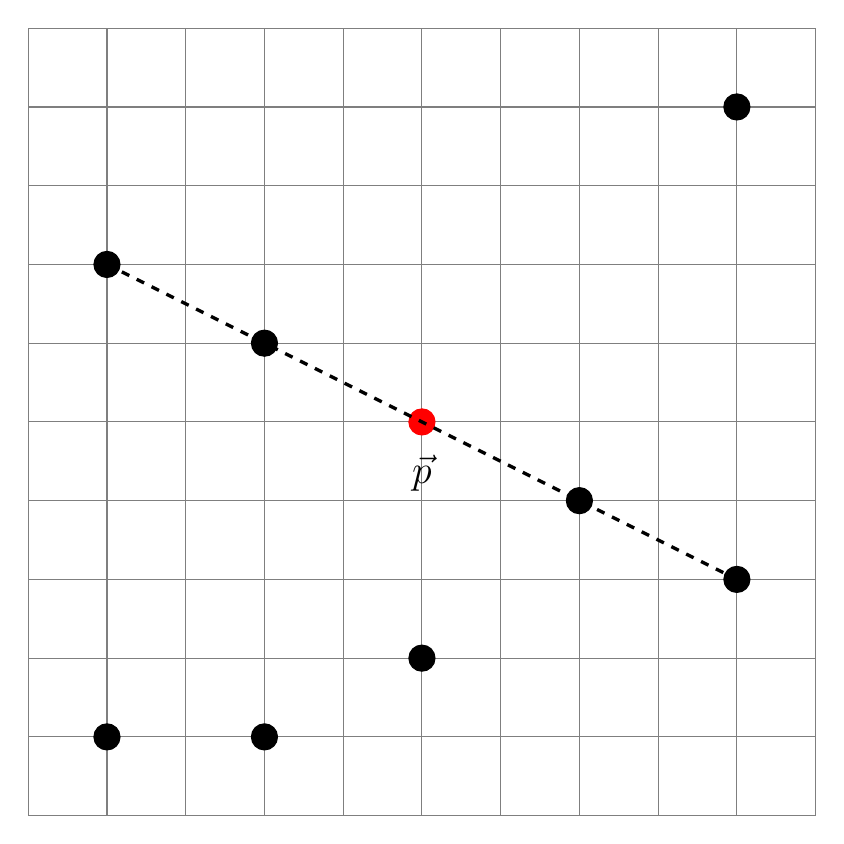
\begin{tikzpicture}

        \draw[opacity=.5] (0,0) grid (10, 10);

        \foreach \x/\y in {%
            3/1,
            5/2,
            3/6,
            1/7,
            7/4,
            9/3,
            9/9,
        }{
            \draw node[draw, fill, minimum width=.1cm, circle] at (\x, \y) {};
        }

        \draw node [draw, fill, minimum width=.1cm, circle, red] at (5, 5) {};
        \draw node[below=.3cm] at (5,5) {\Large $\vec p$};
        \draw[very thick, dashed] (1, 7) -- (9, 3);

    \end{tikzpicture}
    }
    \end{center}

    In a file named \python{max_points_on_line.py}, write a function
    \python{max_points_on_line(X, p)} which accepts the following arguments:
    \begin{itemize}
        \item \python{X}: A list of points, each point being a 2-tuple of integers.
        \item \python{p}: A query point represented as a 2-tuple of integers.
    \end{itemize}
    Your function should return the maximum number of points in \python{X} that fall
    on the same straight line containing $\vec p$. Your answer should be an
    integer. If \python{X} is empty, return \python{0}. If a point $\vec{x}$ in \python{X}
    is such that $\vec x = \vec p$, you should consider to be on the same line as $\vec{p}$
    (even if there are no other points).

    Your algorithm should take expected time that is linear in the number of points in
    \python{X}.

    Example (using the points in the picture above):

    \begin{minted}[autogobble]{python}
    >>> X = [
    ... (1, 1),
    ... (3, 1),
    ... (5, 2),
    ... (3, 6),
    ... (1, 7),
    ... (7, 4),
    ... (9, 3),
    ... (9, 9)
    ... ]
    >>> p = (5, 5)
    >>> max_points_on_line(X, p)
    4
    \end{minted}

    \emph{Hint}: maybe you can use a hash table (i.e., a Python dictionary)?
    Remember, to use hashing in solving an algorithmic problem, you often
    need to turn the problem into a \emph{membership query}. For any given
    point $\vec x$, you can calculate the slope of the line it makes with $\vec
    p$. How can you turn checking to see if there are other points with the
    same slope into a membership query?

    \begin{soln}
        This is an optimization problem that at first might look undoable in a finite
        amount of time: there are infinitely many lines that contain the point $\vec p$,
        and we don't have time to try all of them.

        The key insight is that two points $\vec x_1$ and $\vec x_2$ will fall on the
        same line with $\vec p$ if and only if the slope between $\vec x_1$ and $\vec p$
        is the same as the slope between $\vec x_2$ and $\vec p$. This is a consequence
        of the fact that any line containing $\vec p$ is uniquely determined by its slope.

        Therefore, the solution proceeds by making a dictionary (hash map)
        whose keys are slopes and whose values are integers counting the number of points
        we've seen whose slope with $\vec x$ is equal to the key. We loop through all
        points in \python{X} and compute the slope between each point and $\vec p$.
        We index into the dictionary with this slope and increment the count
        stored. If this new value is the largest so far, we update our idea of
        the maximum.

        Working Python code is below:

        \inputminted{python}{\thisdir/include-solution/max_points_on_line.py}
    \end{soln}

\end{progprob}
